\documentclass[10pt,a4paper]{article}
\usepackage[italian]{babel}
\usepackage[T1]{fontenc}
\usepackage[utf8]{inputenc}
\usepackage[affil-it]{authblk}
\usepackage{lineno,hyperref}
\usepackage{amsmath}
\usepackage{amsfonts}
\usepackage{amssymb}
\usepackage{graphicx}
\begin{document}
\title{Appunti di Artificial Intelligence}

\author{Ivan Masnari%
  \thanks{e-mail: \texttt{ivan.masnari@studenti.unimi.it}}}
\affil{Facoltà di Informatica, UniMi, Milano}

\date{Ultima modifica: \today}
\maketitle
\section{Introduzione}

Dato un qualunque sistema, se disponiamo di un insieme di leggi o regole che lo descrivono completamente (nel caso di un sistema fisico avremmo delle equazioni differenziali) potremmo, in teoria, calcolarne in ogni momento lo stato e, quindi, prevederne l'evoluzione nel tempo. 
Tuttavia, nella vita di ogni giorno capita spesso di non avere a disposizione una conoscenza perfetta di un certo sistema. Tale informazione:
\begin{enumerate}
\item{può mancare.}
\item{possiamo averne una conoscenza approssimata.}
\end{enumerate}
L'intelligenza artificiale nasce con lo scopo di estrarre conoscenza direttamente dai dati in nostro possesso attraverso strumenti automatici. Questo modello si differenzia rispetto alla descrizione \emph{a priori} del sistema, in quanto lo simula per comprenderne \emph{a posteriori} il suo comportamento. Per far questo, è stato utile studiare come gli esseri viventi interagiscano con l'ambiente circostante e come vi si adattino.
Vari modelli di intelligenza artificiale sono stati proposti lungo la storia della disciplina. Una categorizzazione preliminare che si fa in letteratura è quella tra modelli:
\begin{enumerate}
\item{\emph{simbolici}, in cui i dati vengono sottoposti a codifica e solo dopo manipolati. Storicamente questo è stato il primo approccio adottato (vedi sistemi esperti degli anni '70).}
\item{\emph{pre-simbolici}, in cui i dati vengono manipolati direttamente, senza la mediazione di una codifica. Fanno parte di questa famiglia: le reti neurali, i sistemi fuzzy e gli algoritmi evolutivi.}
\end{enumerate}
Nel corso ci concentreremo sui secondi.

\section{Reti neurali}

\subsection{Background biologico}

Il nostro cervello ci permette di analizzare in maniera molto sofisticata l'ambiente in cui ci troviamo per agire nel miglior modo possibile (esempio: se riconosciamo un leone nella savana, scappiamo nell'altra direzione). Queste analisi sono basate sul funzionamento del cervello: come estrae informazioni, come queste interagiscono con l'informazioni contenute in memoria, etc. Lo studio di questi processi è un campo di ricerca molto attivo e multidisciplinare dove convergono gli interessi della biologia, della medicina e della psicologia.
Tali studi ci offrono dei modelli che simulano l'attività celebrale. Proprio questi modelli, vengono poi utilizzati dall'informatica per offrire strumenti di predizione, ottimizzazione e problem-solving in vari campi applicativi (guida automatizzata, smart cities, etc.). Il successo di questi modelli è condizionato dal fatto che il nostro cervello è un potente computer capace di computare in parallelo grandi porzioni di dati. Ma come funziona esattamente?

\begin{figure}
\centering
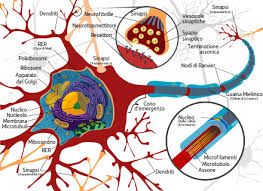
\includegraphics[scale=0.7]{neurone.jpeg}
\caption{Neurone}
\label{fig:1}
\end{figure}

Il cervello è composto da miliardi di cellule dette \emph{neuroni} (Figura \ref{fig:1}). Il neurone a sua volta è costituito da:
\begin{enumerate}
\item{i \emph{dendriti}, i quali sono filamenti raggiunti dalle terminazioni di altri neuroni e che gli permettono di raccogliere informazioni grazie a processi biochimici originati dai così detti \emph{neurotrasmettitori}.}
\item{l'\emph{assone}: un lungo filamento che parte dal corpo centrale della cellula e trasmette segnali elettrici che, a loro volta, vanno ad attivare altri neuroni attraverso il rilascio di neurotrasmettitori.}
\end{enumerate}

Quando e come il neurone trasmetta il segnale di attivazione dipende dal particolare modello fisiologico che si voglia adottare. Solitamente si considera un \emph{threshold}, superato il quale, l'assone viene depolarizzato e la differenza di potenziale provoca il passaggio di una corrente. Un diverso modello prende in considerazione non tanto la potenza dello stimolo quanto il loro numero. 
Questa struttura a network offre ottime prestazioni. Per un confronto con una CPU classica alleghiamo la seguente tabella:

\begin{figure}
\centering
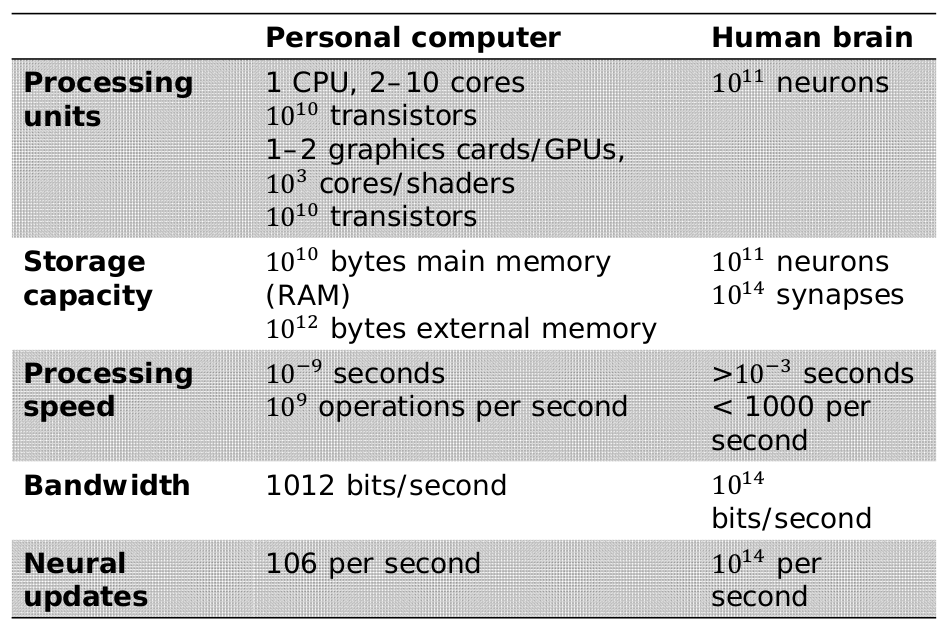
\includegraphics[scale=0.3]{cpuvshuman.png}
\end{figure}

\newpage

I vantaggi delle reti neurali sono:

\begin{enumerate}
\item{alta velocità di calcolo, grazie al parallelismo.}
\item{tolleranza ai guasti: la rete rimane funzionale anche quando molti neuroni smettono di funzionare.}
\item{la performance degrada in modo lineare con il numero di neuroni danneggiati.}
\item{ottimo per l'apprendimento induttivo.}
\end{enumerate}



\section{Sistemi fuzzy}

\section{Algoritmi evolutivi}


\end{document}